% ---------------------------------------------------------------------------------------
\chapter{Dise�o bluetooth}\label{chap2}
En esta secci�n se abordar� el hardware utilizado para prototipado y dise�o de bluetooth bajo consumo (BLE - bluetooth low energy). 

\section{BLEBee}
Para el prototipado se utilizar� un m�dulo bluetooth BLEBee que ofrece una conexi�n simple a placas Arduino que posean este puerto. 
BLEBee utiliza un m�dulo de bluetooth RN4020 el cual ofrece bluetooth versi�n 4.1.\\
Mediante interfaz UART, este modulo puede ser configurado para actuar como m�dulo central o perif�rico cuando establezca una conexi�n.\\
Para conocer mas el funcionamiento de este m�dulo primero hay que conocer mejor la conexi�n XBee.

\begin{figure}[H]
\centering
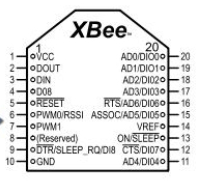
\includegraphics[scale=1]{figura/bluetooth/xbee.png}
\caption{Forma y Pines de puerto XBee}
\label{xbee}
\end{figure}

Como se puede observar en la figura \ref{xbee} el puerto XBee ofrece una conexi�n de 20 pines con usos generales que se utilizan por distintos dispositivos, en este caso bluetooth.\\
En el caso de BLEBee la distribuci�n de los pines se puede observar en la figura \ref{blebee}

\begin{figure}[H]
\centering
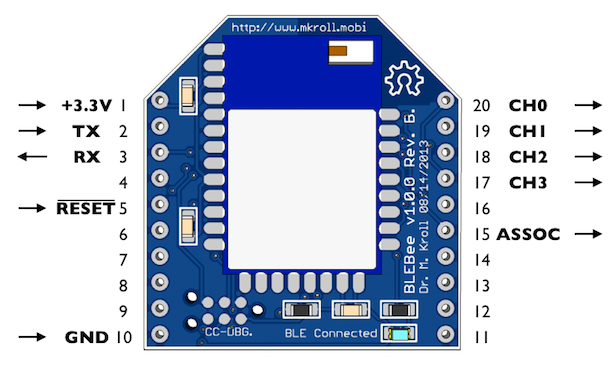
\includegraphics[scale=0.5]{figura/bluetooth/blebee.png}
\caption{Distribuci�n de pines BLEBee}
\label{blebee}
\end{figure}

Comparando la figura \ref{xbee} con la figura \ref{blebee} se puede observar los pines mas relevantes a la hora de dise�ar un m�dulo bluetooth en el dispositivo, siendo los pines mas importantes, y contrastando con el datasheet, los que se muestran en la tabla \ref{pines}

\begin{table}[H]
\centering
\begin{tabular}{| c | c | c |}
\hline
\multicolumn{1}{|c|}{\textbf{N� Pin}}&
\multicolumn{1}{c|}{\textbf{Nombre}}&
\multicolumn{1}{|c|}{\textbf{Descripci�n}}\\ \hline
5  & UART TX & Transmisor UART\\ \hline
6  & UART RX & Receptor UART\\ \hline
7  & WAKE\_ SW & Despertador de modo deep sleep\\ \hline
10 & Led Conexi�n  & Led indicador de conexi�n\\ \hline
12 & Led Actividad & Led indicador de actividad\\ \hline
\end{tabular}
\caption{Pines relevantes m�dulo RN4020}
\label{pines}
\end{table}

\newpage
\section{Comunicaci�n UART}

La comunicaci�n UART (Universal Asynchronous Receiver-Transmitter) es un formato de comunicaci�n serial donde el formato y la velocidad de transmisi�n son configurables. Un UART puede ser un circuito integrado independiente pero en la actualidad vienen incluidos en los microcontroladores.\\
Para entender mejor como funciona la comunicaci�n serial mediante UART hay que observar la figura \ref{UART}

\begin{figure}[H]
\centering
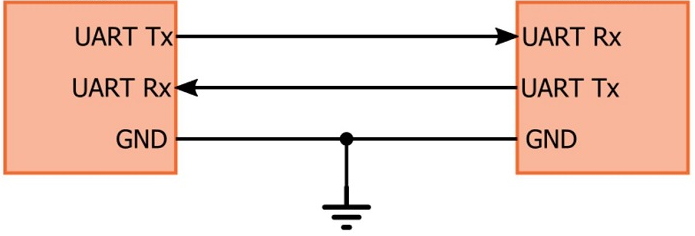
\includegraphics[scale=0.8]{figura/bluetooth/uart.png}
\caption{Configuraci�n para comunicaci�n UART}
\label{UART}
\end{figure}

La comunicaci�n UART cuenta de 2 pines TX (transmisor) y RX (receptor) el cual se conecta al Receptor y transmisor del microcontrolador respectivamente.

\section{Dise�o del m�dulo bluetooth}
Finalmente contrastando lo visto anteriormente y con referente a la tabla \ref{pines} se puede dise�ar el esquem�tico del integrado.\\
Pin 5 y 6 corresponden a la comunicaci�n UART como se explica en la figura \ref{UART}. Es necesario conectar los pines 10 y 12 con diodos led ya que son pines indicadores, el pin 10 indica el estado de la conexi�n con un led verde y tambi�n se recomienda conectar un led azul al pin 12 para ver el estado de actividad (ej. Si se est� enviando informaci�n o est� dormido).\\
El pin 7 cumple la funci�n de despertar el m�dulo bluetooth cuando se encuentre dormido emitiendo desde el microcontrolador una se�al de $3.3[V]$.\\
\begin{figure}[H]
\centering
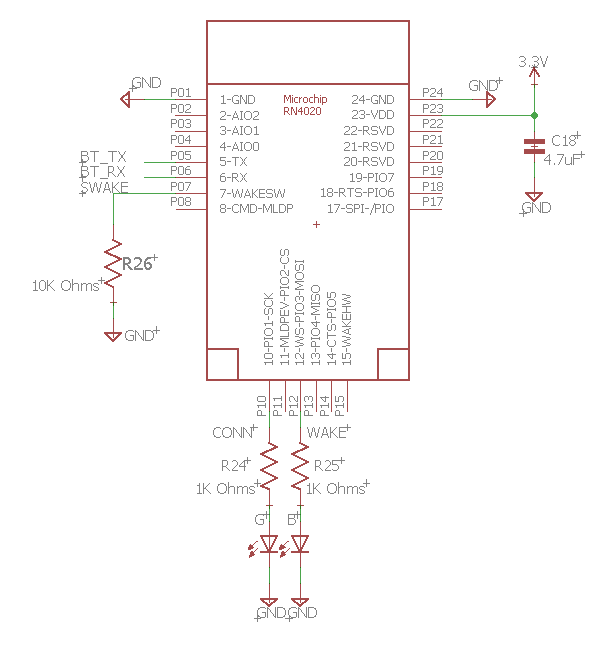
\includegraphics[scale=0.8]{figura/bluetooth/eagle.png}
\caption{Esquem�tico bluetooth dise�ado en EagleCAD}
\label{eagle}
\end{figure}

Como se puede observar en la figura \ref{eagle} se conecta el m�dulo bluetooth con los pines descritos. Se utiliza un condensador en la alimentaci�n de m�dulo para regular el voltaje de la entrada.




